\documentclass{article}
\usepackage{graphicx}
\usepackage{listings}
\usepackage{color}
\usepackage[utf8]{inputenc}

\title{Sperimentazione sulla modellizzazione di una corda vibrante di massa non omogenea\\
	Corso di LSMC, a.a. 2017-2018}
\author{Davide Gori\\
	550282}


\definecolor{backcolour}{rgb}{0.95,0.95,0.92}
\definecolor{gray}{rgb}{0.5,0.5,0.5}
\lstset{basicstyle=\ttfamily\small,
	columns=fullflexible,
	numbers=left,
	numberstyle=\tiny\ttfamily\color{gray},
	backgroundcolor=\color{backcolour},
	tabsize=4,
	language=Octave
}


\begin{document}
	\maketitle
	\section{Obiettivi e descrizione della sperimentazione}
	Vogliamo confrontare la vibrazione di due corde con distribuzione di massa diversa. Confronteremo una corda con massa lineica omogenea con una identica che però presenta un punto "appesantito" da una massa più grande.\\
	Eseguiremo due sperimentazioni, nella prima simuleremo una corda pizzicata dando alla corda posizioni iniziali non nulle e velocità nulla; nella seconda simuleremo una corda colpita da un martelletto diamo velocità non nulle alla corda e posizione iniziale a riposo.

	\section{Prima sperimentazione: corda pizzicata}
	Le corde vengono modellizzate come un vettore di $n=101$ punti distinti i quali esercitano forza elastica ai punti adiacenti ed è presente una forza resistente di attrito. Ogni punto della corda di riferimento ha massa $\frac{10^{-2}}{n}$, i valori delle costanti elastiche sono tutti uguali e valgono $k_i=10^6$ in entrambe le corde, quelli dei coefficienti della forza resistente sono invece $\theta_i=10^{-3}$. Per la seconda corda usiamo gli stessi parametri della prima, salvo modificare la seguente massa $m_51=100*m_1$:\\
	\begin{itemize}
		\item Usiamo lo script {\tt s\_init.m} per impostare le variabili sopra descritte, inoltre poniamo le velocità iniziali a $0$, {\tt pickup} a $20$ (il punto dove registra le vibrazioni), {\tt rate} a $16000$ (numero di campionamenti nel punto di pickup per secondo) e {\tt sec} a $0.1$ (intervallo di tempo di campionamento).
		\item Poniamo $q=5$, cioè impostiamo di pizzicare la corda in quel punto, modificando linearmente le posizioni iniziali in modo che gli estremi siano a quota zero e il punto $q=5$ a quota $1$.
		\item Lo script registra la posizione della corda nel tempo nel punto di pickup grazie alla funzione {\tt suonacorda}, esegue la fft del vettore in output e traccia i grafici di queste. Il grafico delle frequenze della {\tt fft} è ottenuto trascurando le frequenze più alte (che sono frequenze fantasma) e plottando solo la norma, visto che lo sfasamento temporale non è interessante.  
		\item lo script ripete poi il procedimento per la corda modificata come indicato precedentemente.
	\end{itemize}
	
	\section{Lo script}
	Questo è lo script che realizza la sperimentazione:
	
	\lstinputlisting{s_init_1.m}
	
	Dove la funzione {\tt suonacorda} è la sequete:
	
	\lstinputlisting{suonacorda.m}
	
	\section{Risultati}
	
	Riportiamo i grafici della posizione della corda nel tempo (nel punto di pickup) e delle frequenze della fft:
	
	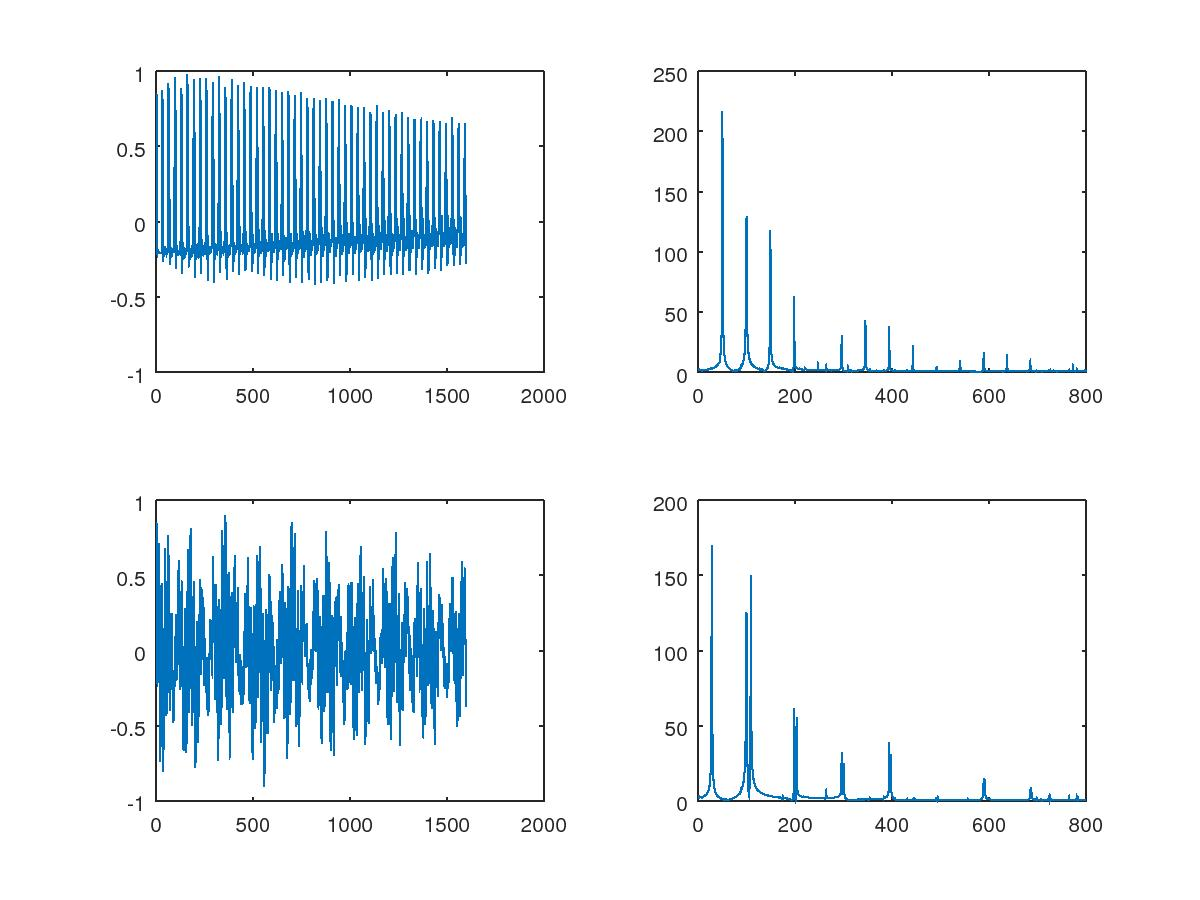
\includegraphics[width=\textwidth]{vib-1.jpeg}
	
	Possiamo notare che nella corda con la massa alterata tutte le frequenze della {\tt fft} sono "sdoppiate". Guardando i grafici della posizione notiamo che nel primo caso la situazione è asimmetrica: questo è dovuto al fatto che la corda non viene pizzicata nel mezzo. Nel secondo caso questo effetto è smorzato dalla presenza della massa più grande che si muove più lentamente.
	
	
	\section{Seconda sperimentazione: corda colpita con martelletto}
	Come prima le corde vengono modellizzate come un vettore di $n=101$ punti distinti i quali esercitano forza elastica ai punti adiacenti ed è presente una forza resistente di attrito. Ogni punto della corda di riferimento ha massa $\frac{10^{-2}}{n}$, i valori delle costanti elastiche sono tutti uguali e valgono $k_i=10^6$ in entrambe le corde, quelli dei coefficienti della forza resistente sono invece $\theta_i=10^{-3}$. Per la seconda corda usiamo gli stessi parametri della prima, salvo modificare la seguente massa $m_51=100*m_1$:\\
	\begin{itemize}
	\item Usiamo lo script {\tt s\_init.m} per impostare le variabili sopra descritte, inoltre poniamo le posizioni iniziali a $0$, {\tt pickup} a $20$ (il punto dove registra le vibrazioni), {\tt rate} a $16000$ (numero di campionamenti nel punto di pickup per secondo) e {\tt sec} a $0.1$ (intervallo di tempo di campionamento).
	\item Poniamo $q=5$, cioè impostiamo di colpire la corda con un martelletto in quel punto, ponendo $v0_{q-j}=10000 exp(-0.01 j^2)$ per $-4 \leq j \leq 4$.
	\item Lo script registra la posizione della corda nel tempo nel punto di pickup grazie alla funzione {\tt suonacorda}, esegue la fft del vettore in output e traccia i grafici di queste. Il grafico delle frequenze della {\tt fft} è ottenuto trascurando le frequenze più alte (che sono frequenze fantasma) e plottando solo la norma, visto che lo sfasamento temporale non è interessante.  
	\item lo script ripete poi il procedimento per la corda modificata come indicato precedentemente.
	\end{itemize}

	\section{Lo script}
	Questo è lo script che realizza la sperimentazione:
	
	\lstinputlisting{s_init_2.m}
	
	Dove la funzione {\tt suonacorda} è la stessa di prima.
	
	\section{Risultati}
	
	Riportiamo i grafici della posizione della corda nel tempo (nel punto di pickup) e delle frequenze della fft:
	
	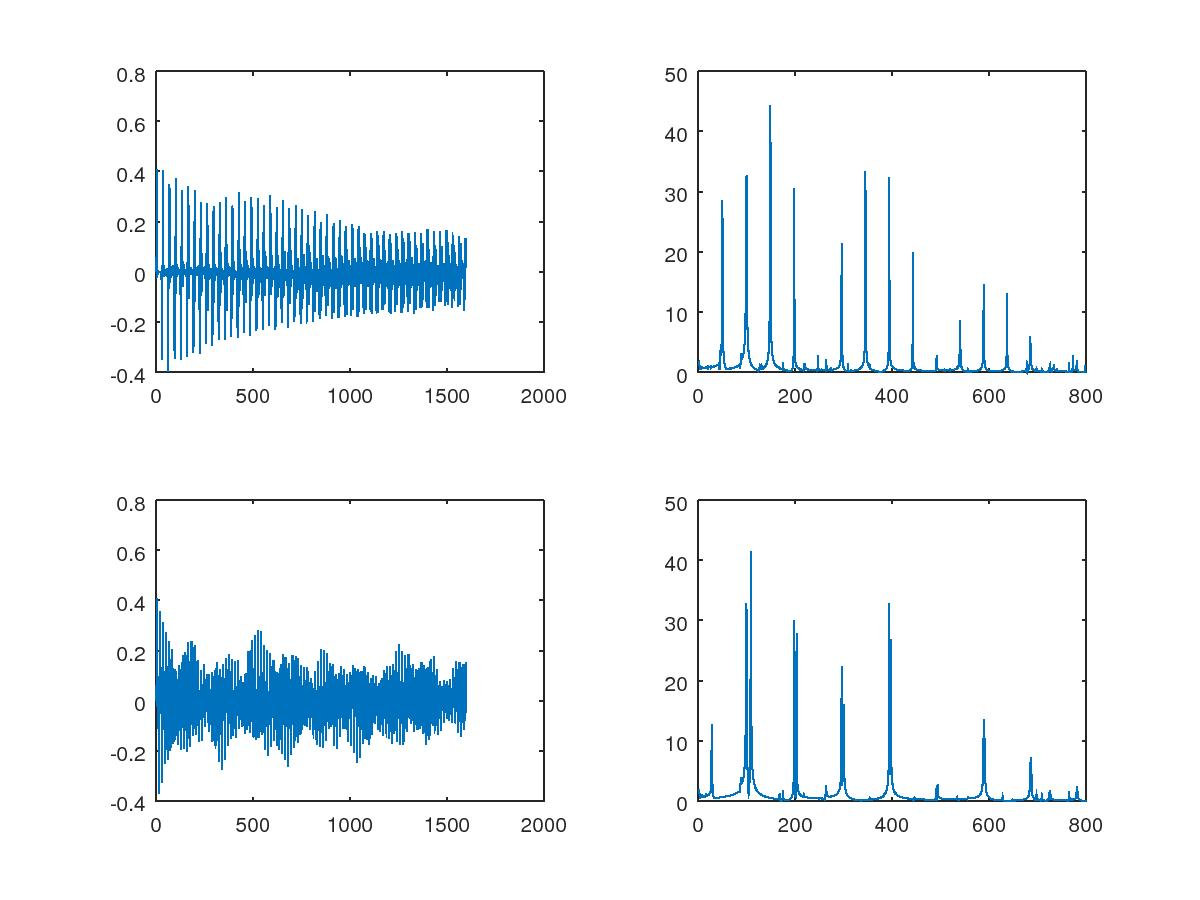
\includegraphics[width=\textwidth]{vib-2.jpeg}
	
	Come prima possiamo notare che nella corda con la massa alterata tutte le frequenze della {\tt fft} sono "sdoppiate". Questo effetto è dovuto dalla presenza della massa più grande che si muove più lentamente.
	quello che mi aspetto: come se massa fosse estremo
	Confrontiamo i grafici
\end{document}